\documentclass[12pt]{article}
\usepackage[margin=0.7in]{geometry} 		% defines page margin
\usepackage{knitting} 				% defines \chart and \textknit
\usepackage{amsmath}
\usepackage{titling} 				% title page
\usepackage{graphicx,xspace, scrextend}	% defines space control stuff
\usepackage{tabularx, array, colortbl}	% defines tables
\usepackage{multicol} 				% defines columns
\usepackage{multirow} 				% defines multirows, combined cells in tables
\usepackage{framed} 				% defines boxes for notes and written directions
\usepackage[x11names]{xcolor} 		% extends color library
\usepackage{hyperref}				% hyperlinks
\hypersetup{
    colorlinks=true,
    linkcolor=blue,
    filecolor=magenta,      
    urlcolor=blue,
}

\pdfmapfile{+knitfont.map}

% font selection
\usepackage{palatino, moresize, sectsty}
\allsectionsfont{\sffamily}

% PICK AND CHOOSE COMMANDS BASED ON NEEDS

\renewcommand{\arraystretch}{2} % compresses tables for pattern keys

\newcolumntype{L}[1]{>{\leftalign\arraybackslash}p{#1}}
\newcolumntype{C}[1]{>{\centering\arraybackslash}p{#1}}

% length parameters
\setlength{\parindent}{0pt} % disables indentation for paragraphs
\setlength{\columnsep}{0.7cm} % column separation in multicol environment

% color parameters
\colorlet{framecolor}{black}
\colorlet{shadecolor}{Snow2}
\colorlet{highlight}{yellow}
\colorlet{wiggle}{lightgray}

% custom commands
\newcommand{\comment}[1]{} % allows for multiline comments that LaTeX will ignore

\newcommand{\vocab}[1]{\emph{\textbf{#1}}} % format for highlighting definitions of stitches, vocabulary terms
\newcommand{\rowDir}[1]{\textbf{#1:}} % indent for written instructions within paragraphs

\renewcommand{\repeat}[1]{\textbf{*[#1]*}} % format for written repeats, bold with *[ stitches ]*
\newcommand{\x}{$\times$}			% times symbol but shorthand
\newcommand{\setrepeat}[2]{\textbf{[#1]}\x{#2}}		% format for repeats with set number of repetitions, bold with [ stitches ]

\newcommand{\blank}{\underline{\hspace{2em}} } % written instructions, fill-in-the-blank box
\newcommand{\highlighted}[1]{\fbox{#1}} % written instructions, highlight particular text
\newcommand{\wiggle}[1]{\fcolorbox{framecolor}{wiggle}{#1}} % highlight in a different color for wiggle room in instructions

% stitch count commands
\newcommand{\increase}[1]{(\emph{+#1 
	\ifnum#1=1{st}\else{sts}\fi})}
\newcommand{\decrease}[1]{(\emph{$-$#1
	\ifnum#1=1{st}\else{sts}\fi})}
\newcommand{\stitchcount}[1]{(\emph{#1 sts})}

% marker instructions
\renewcommand{\pm}[1]{\emph{pm #1}} % place stitch marker
\newcommand{\sm}{\emph{sm}} % slip marker
\renewcommand{\rm}[1]{\emph{rm #1}} % remove stitch marker

% thick horizontal line
\makeatletter \newcommand{\thickhline}{
    \noalign {\ifnum 0=`}\fi \hrule height 1.5pt
    \futurelet \reserved@a \@xhline
}
\makeatother

% custom environments
\newenvironment{frnote}
    {% framed environment for pattern notes
    	\def\FrameCommand{\fboxrule=\FrameRule\fboxsep=\FrameSep \fcolorbox{framecolor}{shadecolor}}
    	\MakeFramed {\advance\hsize-\width\FrameRestore}}
    {\endMakeFramed}

\newenvironment{frdirection}
    {% framed environment for written directions
	\def\FrameCommand{\fboxrule=\FrameRule\fboxsep=\FrameSep \fbox}
   	\MakeFramed {\advance\hsize-\width \FrameRestore}
    	\addmargin[1.5cm]{0pt}}
    {\endaddmargin
	\endMakeFramed}

\newenvironment{unframed}
    {% unframed environment for written directions
	\begin{addmargin}[2em]{0pt}
	\setlength{\parindent}{-2em}}
    {%\vspace{1em}
	\setlength{\parindent}{0em}
	\end{addmargin}}

\title{Play It By Queer (PIBQ)} % pattern name here
\author{Shanel Wu (Piper Nell)}

\begin{document}

%%%%%%%%%%%%%%%%%%%%%%%%%%%%%%%%%%%%%%%%%%%%%%%%%%
% TITLE PAGE 
% COVER PHOTO
% uncommend line below if you want a background fill image
% \ThisLRCornerWallPaper{1.0}{image.jpg} 

% ADD REAL COVER PIC
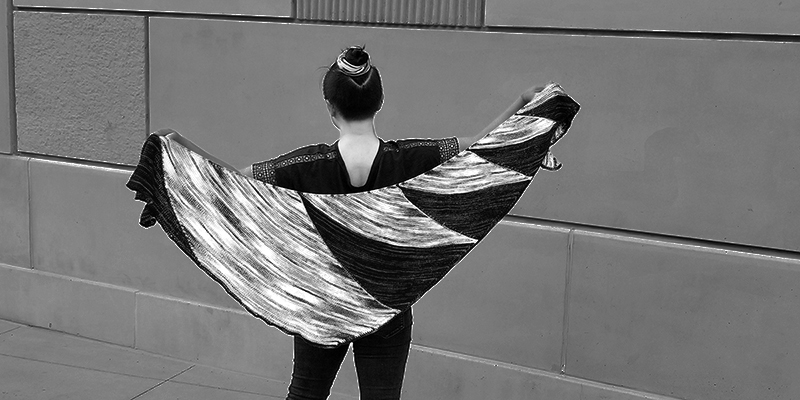
\includegraphics[width=\linewidth]{pics_BW/_spread2}

\vspace{1.5em}

\raggedright
{\fontfamily{qag}\selectfont
\HUGE\textbf{\thetitle} \normalsize
\\\vspace{0.5em}
% adjust this space or use \hfill
\theauthor
}


\begin{multicols}{2}
\small
% Cute description here
When you have that gorgeous single skein that needs to be enjoyed to the last inch, don't overthink it. Just relax and \emph{play it by queer}. 

~\\
Pair your special skein with a contrasting color (or a few colors) and watch them play in soothing garter stitch wedges. The wedges are shaped with short rows, which means that you never work with more than one color at a time.

\subsection*{Yarn Requirements}

% yardage, number of colors, etc.
Two 100g skeins of fingering weight yarn, MC and CC. 
% also include: sample yarn, other yarn suggestions
\emph{Sample used one full skein of Marianated Yarns Practicality Sock (463yds/100g) as MC, and 80g of Manos del Uruguay Alegr\'{i}a (445yds/100g) as CC.} % CC amount?

\subsection*{Needles/Tools}

\begin{itemize}
\item 32" or 40" circular needle in size to obtain fabric of your liking. \emph{Suggested: US5/3.75mm} % NEEDLES
\item stitch markers
\item tapestry needle
\end{itemize}

\vfill ~\\
\columnbreak

\subsection*{Gauge: 5 sts in 1"/2.5cm}

Measured in unblocked, unstretched garter stitch. Not critical for a shawl, but a different gauge may affect yardage required or final size.

~\\
\emph{Sample dimensions after blocking: \\ 73"/186cm tip to tip, 20"/50cm at deepest point}

% sample measurements, gauge, notes on ease, etc.

\subsection*{Techniques}

This pattern is suitable for an advanced beginner. % DIFFICULTY LEVEL
Prior to knitting this pattern, you should be familiar with increasing, decreasing, and short rows. % PREREQUISITE TECHNIQUES
For a complete list of stitches used, see \textbf{Pattern Key}.

% discuss any special techniques and tutorials included

\vfill ~\\
\columnbreak

\subsection*{Pattern Key}

% formatting notes for charts and written directions
In the written instructions, certain numbers will be \highlighted{boxed.} The boxed number reflects the sample, and can be changed to any number you like. Because of this ``wiggle" room, some instructions vary slightly with an odd or even stitch count. If you have an extra stitch, work the instructions in \wiggle{shaded boxes.}

% abbreviation key - fill in with all abbreviations/stitch patterns used in design: written abbreviation, full stitch name or explanation
% try to keep them in sequential order as they appear in the pattern, or in an order that builds upon previous definitions
% chart symbols included in separate keys attached to their respective charts
% stitches with explanations must first be BOLDED, followed by colon then explanation
\begin{center}
{\renewcommand{\arraystretch}{1.2}
\begin{tabular}{| C{0.2\linewidth}  p{0.7\linewidth} | }
\thickhline \rowcolor{shadecolor} 
\textbf{Written}	& \textbf{Description} \\ \thickhline
CO 	& cast on \\
k	& knit \\
st(s)	& stitch(es) \\
RS	& right side \\
WS	& wrong side \\
kfb 	& knit front back \\
sl 	& slip stitch purlwise; \hfill\hfill \linebreak
\textbf{wyib} - ``with yarn in back" \hfill\hfill \linebreak
or \textbf{wyif} - ``with yarn in front" \\
k2tog 	& knit 2 together \\
dst	& \textbf{double stitch:} See \vocab{German Short Rows} note on next page. \\
\hline
\end{tabular}}
\end{center}

\vspace{5em}

\subsection*{Schematic}
% schematic of sample
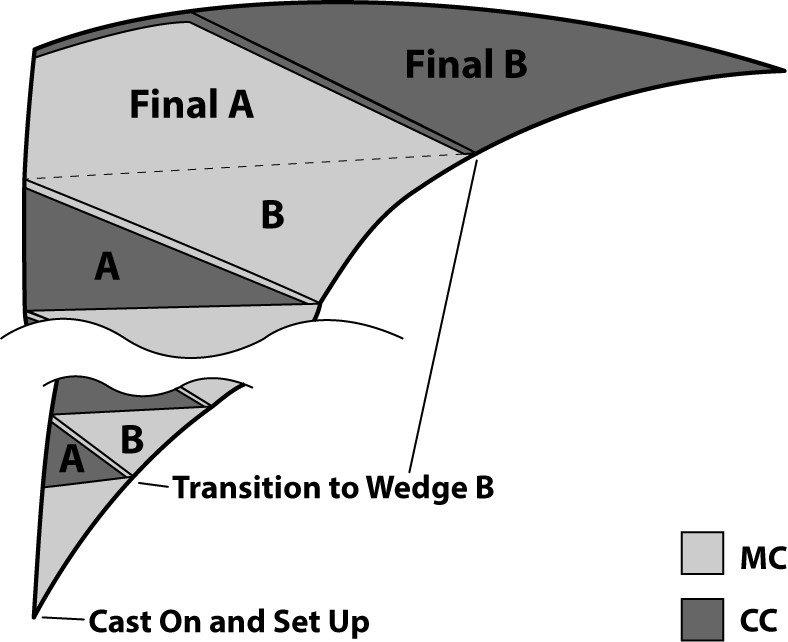
\includegraphics[width=\linewidth]{pics_BW/schematic_sample_BW.png}

\columnbreak

\subsection*{Construction}

The PIBQ is an asymmetrical triangular shawl that begins at one of the points and grows with repeating short row wedges. The wedges are worked in pairs, one in CC (Wedge \textbf{A}) and one in MC (Wedge \textbf{B}). 

~\\
The schematic on this page shows the layout of the cast on section and repeated wedge pairs. When you no longer have enough MC to complete another wedge pair, continue to the Final Wedges (\textbf{Final A} and \textbf{Final B}) where you will use up the remainder of MC.

\begin{frnote}
If you really don't have a lot of MC left for the final wedges, see the \textbf{Color Variations} appendix for an \vocab{Alternate Final Wedges} finish, as well as other ideas for playing with color.
\end{frnote}


\subsection*{Estimating Yarn Usage}

For knitters who prefer to plan out their projects, here is some math. Each wedge pair will use approximately \vocab{twice} as much yarn as the wedges in the previous repeat. For example, if Wedge A in the current repeat uses 10g of yarn, then the next Wedge A will use about 20g. Using this very rough figure, you can budget your yarn and estimate how many repeats to work.

\begin{frnote}
For an even more precise estimate, see the appendix \textbf{Estimating Yarn Usage (Cont.)}
\end{frnote}


\end{multicols}

%%%%%%%%%%%%%%%%%%%%%%%%%%%%%%%%%%%%%%%%%%%%%%%%%%
% BEGIN INSTRUCTIONS
\newpage
\begin{multicols}{2} \normalsize
\section*{1. Cast On and Set Up}

With MC, CO 4 sts. Work Rows 1-10 once.

~\\
\rowDir{Row 1 (RS)} k3, kfb. \stitchcount{5}

\rowDir{Row 2 (WS)} k2, sl3 wyif.

\rowDir{Row 3} k3, kfb, k1. \stitchcount{6}

\rowDir{Row 4} k3, sl3 wyif.

\rowDir{Row 5} k3, kfb, k2. \stitchcount{7}

\rowDir{Row 6} k4, sl3 wyif.

\rowDir{Row 7} k3, kfb, k3. \stitchcount{8}

\rowDir{Row 8} k5, sl3 wyif.

\rowDir{Row 9} k3, kfb, k1, k2tog, k1.

\rowDir{Row 10} k4, kfb, sl3 wyif. \stitchcount{9}

~\\
Work \highlighted{28} \vocab{full ridges}, ending after a WS row.

% FULL RIDGE
\begin{framed}
\vocab{full ridge} \increase{1} \vspace{0.5em}

\rowDir{Row 11 (RS)} k3, kfb, k to 3 sts from end, k2tog, k1.

\rowDir{Row 12 (WS)} k to 4 sts from end, kfb, sl3 wyif.
\end{framed}
\columnbreak

% INSERT PICTURE OF WEDGE PAIR HERE
\hfill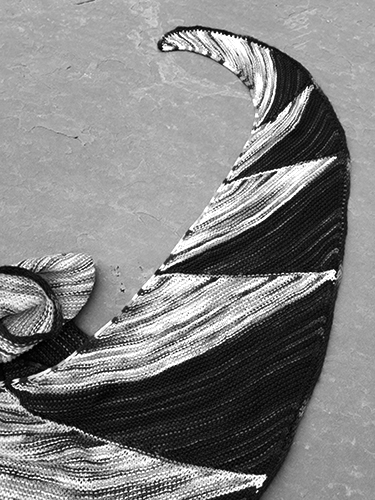
\includegraphics[width=\linewidth]{pics_BW/_COcorner}
\vfill
\end{multicols}

\vfill
\begin{multicols}{2}
% GERMAN SHORT ROW techniques
\begin{frnote} \vspace{-1em}
\subsubsection*{German Short Rows in Garter Stitch}

\emph{I found that German short rows created the neatest finish for the shawl. However, you can substitute another short row method.}

~\\
\rowDir{double stitch (dst)}
Bring yarn forward, slip 1 as if to purl. Pull yarn up, over, and behind the needle to create a \vocab{double st}. Leave yarn in back to knit.

~\\
\rowDir{working a dst}
Insert needle into both loops of the dst as if to knit, k2tog.
\end{frnote}

\columnbreak

\section*{2. Wedge A (CC)}

Join CC (do not break MC). Work Rows 13 and 14 once to set up for Wedge A.

\rowDir{Row 13 (RS)} k3, kfb, k to 3 sts from end, k2tog, k1.

\rowDir{Row 14 (WS)} k to 4 sts from end, turn and dst.

~\\
Work \vocab{short ridges A} until the dst of Row 16 is only 3 \wiggle{or 4} sts from the end of the row. Then, work Rows 17 and 18 once to finish the wedge.

% SHORT RIDGE A
\begin{framed}
\vocab{short ridge A} \decrease{1}\vspace{0.5em}

\rowDir{Row 15} k to 3 sts from end, k2tog, k1.

\rowDir{Row 16} k to 2 sts from previous dst, turn and dst.
\end{framed}

\rowDir{Row 17} \wiggle{k1,} k2tog, k1. \decrease{1}

\rowDir{Row 18} k to 4 sts from end and work all dsts as you come to them, kfb, sl3 wyif. \increase{1}

\newpage

\subsection*{2.1. Transition to Wedge B}

Break CC. Pick up MC to work one \vocab{full ridge}.

% BEGIN WEDGE B
\section*{3. Wedge B (MC)}

Continuing in MC, work Rows 19 and 20 once to set up for Wedge B.

\rowDir{Row 19 (RS)} k3, kfb, k2, turn and dst. \increase{1}

\rowDir{Row 20 (WS)} k to 4 sts from end, kfb, sl3 wyif. \increase{1}

~\\
Work \vocab{short ridges B} until the dst of Row 21 is only 3 \wiggle{or 4} sts from the end of the row.

% SHORT RIDGE B
\begin{framed}
\vocab{short ridge B} \increase{2}\vspace{0.5em}

\rowDir{Row 21} k3, kfb, k to dst, work dst, k2, turn and dst.

\rowDir{Row 22} As Row 20.
\end{framed}

\rowDir{Row 23} k3, kfb, k to dst, work last dst, \wiggle{k1,} \\k2tog, k1.

\rowDir{Row 24} As Row 20. \increase{1}

~\\
Repeat Wedges A and B until you do not have enough MC to complete another Wedge B.

% FINAL WEDGES
\section*{4. Final Wedges}

\subsection*{Final Wedge A}

Continuing in MC, begin Wedge A with Rows 13 and 14. Work \vocab{short ridge A} until you are almost out of MC. Place a stitch marker before beginning the next row. Work Row 15 once more, then Row 18 to finish the final Wedge A.

\subsection*{Final Wedge B}

Join CC. Work Rows 11 and 12 for the usual transition to Wedge B, slipping the marker when you come to it. Set up with Rows 19 and 20. Work \vocab{short ridge B} until there are only 3 sts between the dst of Row 21 and the marker. Work one last \vocab{full ridge}, working the dst's and removing the marker as they come.

\columnbreak

\section*{5. Bind Off}

\emph{You can substitute an applied i-cord edging. I just prefer to pick up all the stitches at once!} \vspace{-1em}

\subsection*{Pick Up Edge Sts}
\rowDir{Next RS row} k3, kfb, k to end. \increase{1} At the end of the row, do not turn work. Instead, with RS facing, pick up and knit 1 st from every garter ridge on the left selvedge. When you reach the CO corner of the piece, turn to WS. \\
\rowDir{Next WS row} Starting from the rightmost stitch, pick up and knit 3 sts in CO edge of the i-cord border as shown below. Slip these sts wyib back to the left needle.

\begin{center}
\vspace{-2em}
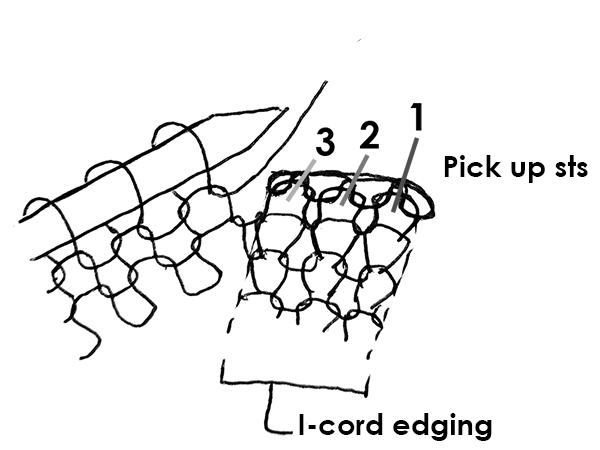
\includegraphics[height=2.5in]{pics_BW/pickup.png}
\end{center}

Bind-off sts on RS as follows, until there are 6 sts left on the needle.

\begin{framed}
\rowDir{I-cord Bind-off} k2, k2tog. Keeping yarn in back, slip the 3 sts on right needle back to the left needle. \decrease{1}
\end{framed}

At the end of the bind-off, graft the first 3 sts to the last 3 sts as shown below.

\vspace{-1em}
\begin{center}
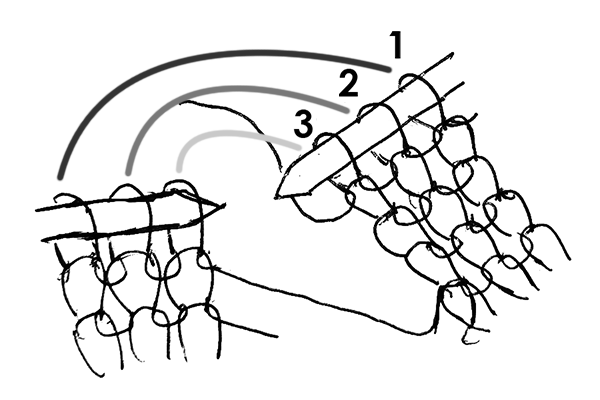
\includegraphics[height=2in]{pics_BW/kitchener.png}
\end{center}

\newpage

\subsection*{Finishing}

Weave in ends and block into desired shape. The corner can be pinned into a point or rounded out as a curve.

~\\
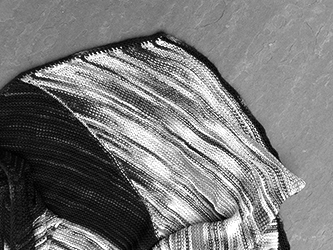
\includegraphics[width=\linewidth]{pics_BW/_middlepoint}

%%%%%%%%%%%%%%%%%%%%%%%%%%%%%%%%%%%%%%%%%%%%%%%%%%
% APPENDICES (IF ANY)

\section*{+ Estimating Yarn Usage (Cont.)}

To calculate a more accurate ratio for how your wedges increase in size, measure how much yarn your 1st and 2nd Wedge A's use, then insert into the below formula.

\vspace{-1em}
{\renewcommand{\arraystretch}{1.0}
\[
\left.\begin{matrix}
\text{2nd Wedge A} \\ 
\framebox(80,24){\hfill g~}
\end{matrix}\right.
\begin{matrix}\vspace{-1em}\\\div\end{matrix}
\left.\begin{matrix}
\text{1st Wedge A} \\ 
\framebox(80,22){\hfill g~}
\end{matrix}\right.
\begin{matrix}\vspace{-1em}\\=\end{matrix}
\left.\begin{matrix}
\text{ratio} \\ 
\framebox(50,22){~}
\end{matrix}\right.
\]}

The following table can be used for predicting or tracking yarn consumption.

\begin{center} \renewcommand{\arraystretch}{1.5}
\begin{tabular}{| C{0.1\linewidth} | C{0.2\linewidth} | C{0.2\linewidth} |}
\thickhline \rowcolor{shadecolor} 
\#	& A 	& B 	\\ \thickhline
1	& \blank g	& \blank g	\\
2	& \blank g	& \blank g	\\
3	& \blank g	& \blank g	\\
4	& \blank g	& \blank g	\\
5	& \blank g	& \blank g	\\
6	& \blank g	& \blank g	\\
7	& \blank g	& \blank g	\\ \hline
\end{tabular}\end{center}
\columnbreak

\section*{+ Color Variations}

\subsection*{Alternative Final Wedges}

Work Wedge A as normal, then work transition in CC. Begin Wedge B with MC, then switch to CC when MC runs out.

~\\
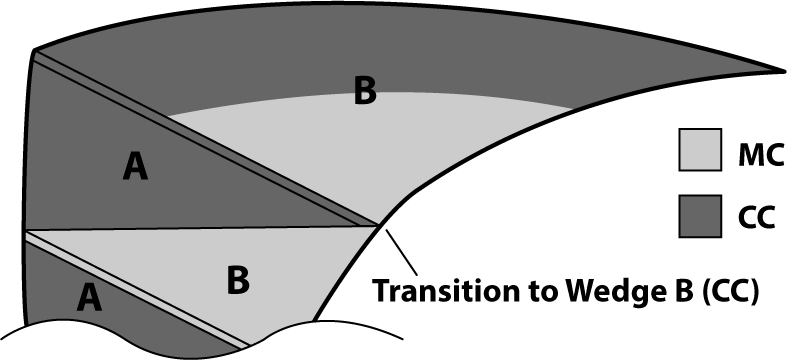
\includegraphics[width=\linewidth]{pics_BW/schematic_sample2_BW}

\subsection*{Make Your Own!}
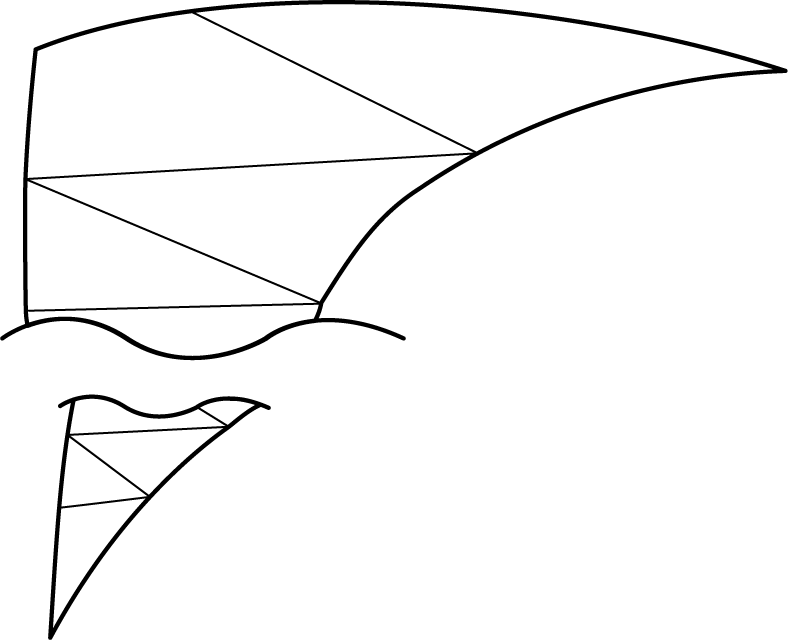
\includegraphics[width=\linewidth]{schematic_template}


\vfill ~\\

%%%%%%%%%%%%%%%%%%%%%%%%%%%%%%%%%%%%%%%%%%%%%%%%%%
% COPYRIGHT

\begin{frnote} \ssmall
Pattern \& photos \copyright  2019 Shanel Wu.
All rights reserved. In purchasing this pattern, you agree to print and use this pattern only for personal use. Do not redistribute or sell paper or electronic copies of this pattern.
\end{frnote}

\end{multicols}
\end{document}